\documentclass[conference]{IEEEtran}
\IEEEoverridecommandlockouts
% The preceding line is only needed to identify funding in the first footnote. If that is unneeded, please comment it out.
\usepackage{cite}
\usepackage{amsmath,amssymb,amsfonts}
\usepackage{algorithmic}
\usepackage{graphicx}
\usepackage{textcomp}
\usepackage{xcolor}
\def\BibTeX{{\rm B\kern-.05em{\sc i\kern-.025em b}\kern-.08em
    T\kern-.1667em\lower.7ex\hbox{E}\kern-.125emX}}
\begin{document}

\title{Autonomous Driving in a Roundabout}

\author{\IEEEauthorblockN{1\textsuperscript{st} Given Name Surname}
\IEEEauthorblockA{\textit{dept. name of organization (of Aff.)} \\
\textit{name of organization (of Aff.)}\\
City, Country \\
email address or ORCID}
\and
\IEEEauthorblockN{2\textsuperscript{nd} Given Name Surname}
\IEEEauthorblockA{\textit{dept. name of organization (of Aff.)} \\
\textit{name of organization (of Aff.)}\\
City, Country \\
email address or ORCID}
}

\maketitle

\begin{abstract}
While intersection are often used as the classic test case for interaction in autonomous driving, a roundabout is another interesting case where multiple agents interact. In this paper we study the optimal policy for navigating a roundabout and how it changes when some agents break the rules of the road. We show that unsafe participants in the roundabout lower its throughput by forcing the autonomous driving agent to adopt a more conservative policy.
\end{abstract}

%\begin{IEEEkeywords}
%\end{IEEEkeywords}

\section{Introduction}
Roundabouts are relatively uncommon compared to intersections in the US, %\citation needed
but are rising in popularity due to their fuel and time saving benefits. Unfortunately many human drivers do not know how to navigate a roundabout, limiting their utility. We are interested in two questions:
\begin{itemize}
	\item Can we train an RL agent to successfully navigate a roundabout?
	\item How does the optimal policy change when unsafe drivers are present in the roundabout?
\end{itemize}

\section*{Problem Description}
We represent this problem as a Markov decision process (MDP) over discrete states and actions. 

\subsection*{States} We define three integer-valued states: $s_1$, $s_2$ and $s_3$.
$s_1$ has three values: if $s_1 = 1$, the vehicle has not entered the roundabout, if $s_1=2$, the vehicle is in the roundabout, and if $s_1=3$, the vehicle has passed the roundabout.
 
$s_2$ is the distance between the ego vehicle and the closest vehicle ``in front", approximating the closest vehicle that reasonably presents a collision risk. This distance ranges from $0$ to $10$. %TODO diagram.

$s_3$ is the ego vehicle velocity, sorted into buckets from $0$ to $10$.

\subsection*{Actions} Our RL agent has three actions available: \verb|ZERO| (no acceleration action), \verb|ACCEL| and \verb|DECEL|. Lane-keeping is managed separately to simplify the problem, and no lane changes take place.

With this representation, there are $|S_1|\times|S_2|\times|S_3| = 363$ states and 3 actions. This is a small problem, so it is possible to learn an optimal policy by a direct method such as Bellman iteration.

\subsection*{Reward} The RL agent receives a time-based reward $10 + (N-t)$ for reaching its goal on the other side of the roundabout, where $N$ is the number of time steps in the simulation and $t$ is the step where the goal is reached. This incentivizes quickly crossing the roundabout.

If a collision occurs, the agent receives a reward of $-1000$ and the simulation stops.

\section*{Modeling Other Drivers}
To provide other agents for the simulation, we defined two fixed policies by observing human drivers at the Manzanita Field roundabout.
\subsection*{Safe Driver Model} The safe driver model approximates the correct way to navigate a roundabout: when approaching, it yields to traffic already in the roundabout. If another vehicle is too close, it decelerates unless said vehicle is not currently in the roundabout (assuming the other driver should yield).

Otherwise, it prefers to maintain a constant speed.
\subsection*{Unsafe Driver Model}
The unsafe driver model behaves like the safe driver model with probability $p \in [0,1]$. With probability $1-p$ it may take a rule-breaking action such as:
\begin{itemize}
	\item Yielding to a vehicle waiting to enter the roundabout.
	\item Not yielding to another vehicle when entering the roundabout.
\end{itemize}
\begin{figure}[h]
	\centering
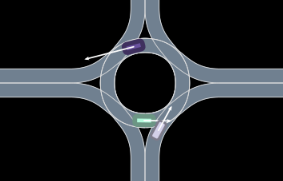
\includegraphics[width=0.7\linewidth]{figures/unsafe.png}
\caption{The unsafe driver (gray) enters the roundabout in front of the rule-following green car, causing a collision.}
\label{fig:unsafe}
\end{figure}

\section{Methodology}
We used online Bellman iteration to learn the roundabout policy by repeatedly running the simulation with randomly chosen starting positions and other drivers.
We studied two cases:

\subsection*{All safe drivers:} The other drivers all follow the rules, yielding and proceeding correctly. Since Bellman iteration is exact, this should converge to an optimal policy for navigating the roundabout.

\subsection*{Some unsafe drivers:} A fraction $r\in (0,1)$ of the drivers break the rules.

\section{Results}

%\subsection{Figures and Tables}
%\paragraph{Positioning Figures and Tables} Place figures and tables at the top and 
%bottom of columns. Avoid placing them in the middle of columns. Large 
%figures and tables may span across both columns. Figure captions should be 
%below the figures; table heads should appear above the tables. Insert 
%figures and tables after they are cited in the text. Use the abbreviation 
%``Fig.~\ref{fig}'', even at the beginning of a sentence.
%
%\begin{table}[htbp]
%\caption{Table Type Styles}
%\begin{center}
%\begin{tabular}{|c|c|c|c|}
%\hline
%\textbf{Table}&\multicolumn{3}{|c|}{\textbf{Table Column Head}} \\
%\cline{2-4} 
%\textbf{Head} & \textbf{\textit{Table column subhead}}& \textbf{\textit{Subhead}}& \textbf{\textit{Subhead}} \\
%\hline
%copy& More table copy$^{\mathrm{a}}$& &  \\
%\hline
%\multicolumn{4}{l}{$^{\mathrm{a}}$Sample of a Table footnote.}
%\end{tabular}
%\label{tab1}
%\end{center}
%\end{table}
%
%\begin{figure}[htbp]
%\centerline{\includegraphics{fig1.png}}
%\caption{Example of a figure caption.}
%\label{fig}
%\end{figure}
%
%Figure Labels: Use 8 point Times New Roman for Figure labels. Use words 
%rather than symbols or abbreviations when writing Figure axis labels to 
%avoid confusing the reader. As an example, write the quantity 
%``Magnetization'', or ``Magnetization, M'', not just ``M''. If including 
%units in the label, present them within parentheses. Do not label axes only 
%with units. In the example, write ``Magnetization (A/m)'' or ``Magnetization 
%\{A[m(1)]\}'', not just ``A/m''. Do not label axes with a ratio of 
%quantities and units. For example, write ``Temperature (K)'', not 
%``Temperature/K''.

\section*{Acknowledgments and Future Work}
I would like to thank Prof. Kochenderfer and all of his TAs for being great this quarter, teaching a lot of interesting material and giving us the freedom to try something on our own with our final projects.

SISL developed the AutomotiveSimulator.jl package which provided a reliable base for RL training and simulations.

Finally, my original proposal was to use MDPs for modeling intersections. Credit for the switch to a more interesting topic goes to all of the sub-optimal drivers holding up traffic in Stanford's roundabouts.
%\section*{References}

%Please number citations consecutively within brackets \cite{b1}. The 
%sentence punctuation follows the bracket \cite{b2}. Refer simply to the reference 
%number, as in \cite{b3}---do not use ``Ref. \cite{b3}'' or ``reference \cite{b3}'' except at 
%the beginning of a sentence: ``Reference \cite{b3} was the first $\ldots$''
%
%Number footnotes separately in superscripts. Place the actual footnote at 
%the bottom of the column in which it was cited. Do not put footnotes in the 
%abstract or reference list. Use letters for table footnotes.
%
%Unless there are six authors or more give all authors' names; do not use 
%``et al.''. Papers that have not been published, even if they have been 
%submitted for publication, should be cited as ``unpublished'' \cite{b4}. Papers 
%that have been accepted for publication should be cited as ``in press'' \cite{b5}. 
%Capitalize only the first word in a paper title, except for proper nouns and 
%element symbols.
%
%For papers published in translation journals, please give the English 
%citation first, followed by the original foreign-language citation \cite{b6}.

\begin{thebibliography}{00}
%\bibitem{b1} G. Eason, B. Noble, and I. N. Sneddon, ``On certain integrals of Lipschitz-Hankel type involving products of Bessel functions,'' Phil. Trans. Roy. Soc. London, vol. A247, pp. 529--551, April 1955.
%\bibitem{b2} J. Clerk Maxwell, A Treatise on Electricity and Magnetism, 3rd ed., vol. 2. Oxford: Clarendon, 1892, pp.68--73.
%\bibitem{b3} I. S. Jacobs and C. P. Bean, ``Fine particles, thin films and exchange anisotropy,'' in Magnetism, vol. III, G. T. Rado and H. Suhl, Eds. New York: Academic, 1963, pp. 271--350.
%\bibitem{b4} K. Elissa, ``Title of paper if known,'' unpublished.
%\bibitem{b5} R. Nicole, ``Title of paper with only first word capitalized,'' J. Name Stand. Abbrev., in press.
%\bibitem{b6} Y. Yorozu, M. Hirano, K. Oka, and Y. Tagawa, ``Electron spectroscopy studies on magneto-optical media and plastic substrate interface,'' IEEE Transl. J. Magn. Japan, vol. 2, pp. 740--741, August 1987 [Digests 9th Annual Conf. Magnetics Japan, p. 301, 1982].
%\bibitem{b7} M. Young, The Technical Writer's Handbook. Mill Valley, CA: University Science, 1989.
\end{thebibliography}

\end{document}
